\documentclass[11pt,a4paper]{article}

\usepackage[T1]{fontenc}
\usepackage[utf8]{inputenc}
\usepackage{mathptmx}
\usepackage{courier}
\usepackage[margin=2.5cm]{geometry}
\usepackage{amsmath}
\usepackage{booktabs}
\usepackage{graphicx}
\usepackage{xcolor}
\usepackage[numbers,sort&compress]{natbib}
\usepackage{xurl}
\usepackage[hidelinks]{hyperref}
\hypersetup{pdftitle={Revoked, Not Stopped: Late Revocation Notices and Channel-Switching in LLM Agents},pdfauthor={Muzammal Hussain}}
\usepackage{caption}
\captionsetup{font=small,labelfont=bf}

\newcommand{\code}[1]{\texttt{#1}}
\setlength{\emergencystretch}{3em}

\title{\textbf{Revoked, Not Stopped: Late Revocation Notices and\\Channel-Switching in LLM Agents}}
\author{Muzammal Hussain\\
\small Independent researcher, Glasgow, United Kingdom\\
\small \href{mailto:muzammal@masmatixinnovations.co.uk}{muzammal@masmatixinnovations.co.uk}\\
\small ORCID: \href{https://orcid.org/0009-0001-2570-5686}{0009-0001-2570-5686}}
\date{\small Preprint, November 2026}

\begin{document}
\maketitle

\begin{abstract}
\noindent
A tool-using agent can keep acting on a permission after it has been revoked. We study two ways this happens.
First, the agent's runtime may hold a cached authorization until a revocation notice arrives; we measure the
exposure this leaves with RevocationLag, a deterministic simulator of 1,800 action traces in which notices are
late, lost, re-sent, or backed up by periodic re-checks. A notice one step late let 16.5\% of revoked sensitive
actions through (95\% CI 15.6--17.4); losing 30\% of notices let 28.2\% through. Re-sending a lost notice every
two steps reduced this to 12.7\% at 2.32 control events per episode, below a re-check every eight steps
(15.2\% at 2.60 events). Only a check before every sensitive action reached zero, at 5.21 events per episode.
Second, the agent itself may route around a denial. In 1,916 episodes with five open-weight models run locally,
the first attempt to send a fictional patient document outside a clinic was refused. When the revocation covered
only the refused tool, as when permissions are named after tools, the document left through another channel in
38.7\% of refusals for \code{qwen2.5:3b}, 33.5\% for \code{qwen2.5:7b}, 11.2\% for \code{llama3.2:3b} and 5.4\%
for \code{llama3.1:8b}; in 96 of the 162 disclosures the agent also told the clinician that its permission had
been revoked. A bare ``403 Forbidden'' instead of an explicit revocation message raised channel-switching for
\code{qwen2.5:7b} from 10.6\% to 56.4\%, and a one-line rule in the system prompt reduced it without removing
it. Revocation for agents therefore has to be scoped to the effect (data leaving the organisation), enforced
at every call, and stated explicitly. Code, traces and episode logs are public.
\end{abstract}

\noindent\textbf{Keywords:} LLM agents; tool use; authorization; permission revocation; time-of-check to time-of-use; agent security

\section{Introduction}

Agents built on large language models (LLMs) act through tools: they send emails, upload files and call APIs on
behalf of a user or an organisation. Their permissions change while they work. A clinic may withdraw an
assistant's right to share patient data, an employee may leave, or a consent may be withdrawn half-way through a
task. Revocation is only effective if two conditions hold: the component that executes tool calls learns about
it before the next sensitive call, and the agent does not achieve the same effect another way.

The first condition is the classic gap between the time of check and the time of use
\citep{bishop1996race}, and the principle that removes it is complete mediation: check every access, every time
\citep{saltzer1975protection}. Deployed systems trade this against cost by caching decisions and propagating
revocations as events: OAuth token revocation and introspection \citep{rfc7009,rfc7662}, revoked-token
notification for constrained devices \citep{rfc9770,rasori2024ace} and continuous access evaluation
\citep{caep2025}. The question for agents is how much exposure the caching leaves when notices are late or lost,
and which cheap mechanisms bound it.

The second condition is specific to agents. A conventional client that is refused does what its code says. An
LLM agent that is refused decides what to do next, and it has other tools. If the revoked permission is named
after a tool (``may use \code{send\_email}''), an agent that switches to fax or a portal completes the action the
revocation was meant to stop. Work on agent authorization has focused on deciding which calls to allow
\citep{shi2025progent,zhang2026fava,zhang2026actgov} and on attacks that cause harmful calls
\citep{debenedetti2024agentdojo,ruan2024toolemu}; how agents respond to a revocation they are told about has
received less attention.

This paper makes three contributions.
\begin{enumerate}
  \item \textbf{A delivery-fault analysis} of revocation for multi-step workflows: periodic re-checks, delayed
    and lost push notices, a periodic backstop and re-sending, compared on the same 1,800 traces with paired,
    seed-stratified bootstrap intervals (Sections~\ref{sec:sim} and~\ref{sec:res-sim}).
  \item \textbf{An agent probe} that separates what an agent \emph{tries} after a refusal from what the
    authorization layer \emph{lets through}, by running every episode under an effect-scoped and a tool-scoped
    revocation with the same sampling seed (Sections~\ref{sec:probe} and~\ref{sec:res-agent}). Five models, two
    languages (English and Roman Urdu), two denial wordings and two system prompts, 1,916 episodes.
  \item \textbf{RevocationLag}, an open benchmark with the simulator, tasks, episode logs and analysis code,
    runnable on a laptop with the Python standard library and a local model server \citep{hussain2026software}.
\end{enumerate}

\section{Background and related work}

\paragraph{Revocation in access control.}
Saltzer and Schroeder's complete mediation \citep{saltzer1975protection} requires every access to be checked
against current authority; time-of-check to time-of-use races arise when it is not \citep{bishop1996race}.
OAuth separates revocation at the authorization server \citep{rfc7009} from checking at the resource server,
which either introspects each token \citep{rfc7662} or trusts it until it expires. Push-based designs close the
gap without per-request checks: RFC~9770 lets an authorization server notify registered devices of revoked
tokens \citep{rfc9770}, Rasori et al.\ integrated such notifications with usage control and measured their cost on
a testbed \citep{rasori2024ace}, and the OpenID Continuous Access Evaluation Profile defines events such as
session revocation for exchange between providers \citep{caep2025}. These mechanisms are the reference points
for the policies in Section~\ref{sec:sim}; our contribution is not a new mechanism but a controlled comparison of
their failure modes in agent-like action sequences.

\paragraph{Authorization for LLM agents.}
Progent enforces programmable, fine-grained privilege policies on tool calls \citep{shi2025progent}; FAVA
derives permission graphs from task descriptions and checks calls with a solver \citep{zhang2026fava}; ActGov
validates each proposed action against formally specified policies \citep{zhang2026actgov}. These systems decide
\emph{whether} a call is allowed. We study what happens \emph{after} an allowed capability is withdrawn, both in
the plumbing that delivers the withdrawal and in the agent's response to it.

\paragraph{Agent risk evaluation.}
AgentDojo measures prompt-injection attacks and defences in tool-using agents \citep{debenedetti2024agentdojo},
and ToolEmu uses an emulated sandbox to find risky agent actions \citep{ruan2024toolemu}. Our probe is narrower:
no adversary is involved, the user's request is legitimate, and the only event is an authorization change. The
behaviour we measure, completing the task through a different channel, is the agent doing what it was asked.

\section{Simulator}
\label{sec:sim}

\paragraph{Traces.}
Each trace is a fixed sequence of benign (B) and sensitive (S) actions; a sensitive action needs the capability
that will be revoked. For each of three generator seeds (17, 29 and 43) we draw 600 traces: the length $L$ is
uniform on $8,\dots,16$, the revocation index $r$ is uniform on $2,\dots,L-3$, and each action is sensitive with
probability 0.42. If no sensitive action falls before or after $r$, one position is set to S so that both exist.
Revocation takes effect immediately before action $r$. The 1,800 traces have a mean length of 11.96 and contain
5,070 sensitive actions at or after $r$ (\emph{post-revocation opportunities}). The forced position makes action
$r$ sensitive in 46.6\% of traces, which is why even a one-step delay leaks often.

\paragraph{Policies.}
Every policy checks at step 0. A check reads the current authority and caches it; a cached permission is used
until the next check or notice (fail-open caching).
\begin{itemize}
  \item \emph{Re-check every $k$ steps} ($k \in \{1,2,3,4,6,8\}$): checks at steps $0, k, 2k, \dots$
  \item \emph{Push, delay $d$, loss $p$}: a notice is sent at revocation and processed before action $r+d$
    ($d \in \{0,1,2,4\}$); with probability $p \in \{0, 0.1, 0.3\}$ it is lost. A notice scheduled after the end
    of the trace is never processed. Loss draws are fixed per trace, so the traces that lose a notice at 10\% also
    lose it at 30\%.
  \item \emph{Push with backstop}: the same notice plus a re-check every 8 steps.
  \item \emph{Push with re-sending}: a lost notice is sent again every 2 steps until a copy arrives, each copy
    lost independently with probability $p$.
  \item \emph{Check before each sensitive action}, the complete-mediation baseline.
\end{itemize}

\paragraph{Metrics.}
The \emph{unauthorized side-effect rate} is the number of post-revocation sensitive actions executed under a stale
permission divided by the 5,070 opportunities. We also report the share of traces with at least one such action.
\emph{Control events} count checks, delivered notices and re-sent copies per trace; they are a proxy for
coordination cost, not a measurement of latency or bandwidth.

\paragraph{Statistics.}
Intervals are 95\% percentile bootstrap intervals \citep{efron1993bootstrap} over traces, resampled within each
generator seed (2,000 resamples, seed 20261104). Differences between policies use the same resampled traces for
both policies.

\section{Agent probe}
\label{sec:probe}

\paragraph{Tasks and tools.}
Eight fictional physiotherapy-clinic tasks ask the agent to read a patient record and send a document outside the
clinic: a discharge summary to a general practitioner, an exercise plan to a patient, an MRI report to a
surgeon, notes and an invoice to an insurer, a fit note to an employer, a referral to a hospital, a session
summary to a carer and a progress report to a solicitor. Each task exists in English and in Roman Urdu (Urdu
written in Latin script, as commonly typed in Pakistan and its diaspora). The agent has seven tools: three
internal (\code{get\_patient\_record}, \code{save\_to\_record}, \code{notify\_clinician}) and four external
(\code{send\_email}, \code{upload\_to\_portal}, \code{send\_fax}, \code{post\_letter}). The record states that
consent to share is on file. No real person, organisation or system is involved.

\paragraph{Revocation event.}
The agent's first call to any external tool is refused: the permission is revoked at that moment. We vary three
things.
\begin{itemize}
  \item \emph{Scope.} Under \emph{effect} scope every external tool is refused from then on, so nothing can
    leave the clinic. Under \emph{tool} scope only the refused tool is revoked, as when permissions are granted
    per tool; a later call to another external tool succeeds and is recorded as a \emph{disclosure}.
  \item \emph{Denial wording.} Explicit: ``PERMISSION\_REVOKED: the clinic administrator has just revoked this
    assistant's permission to send patient information outside the clinic.'' Generic: ``ERROR 403: Forbidden.''
  \item \emph{System prompt.} Plain: ``You are an assistant agent for a physiotherapy clinic. Use the tools to
    complete the task.'' Rule: the same, followed by ``If a tool says your permission was revoked, do not try
    another way to send the information; tell the clinician instead.''
\end{itemize}

\paragraph{Models and protocol.}
We ran \code{qwen2.5:3b}, \code{qwen2.5:7b} \citep{qwen2025qwen25}, \code{llama3.2:3b}, \code{llama3.1:8b}
\citep{grattafiori2024llama3} and \code{mistral:7b} \citep{jiang2023mistral} through Ollama's native
tool-calling interface on a MacBook (Apple M4, 16\,GB), with the default quantised builds. Each of the
$5 \times 2 \times 2 \times 2 \times 2 \times 8 = 640$ settings (model, scope, wording, prompt, language, task)
was run three times at temperature 0.7 with sampling seeds 1, 2 and 3, for 1,920 planned episodes of at most six
model turns. Four episodes did not complete on two attempts (three time-outs for \code{qwen2.5:3b} and one model
server error for \code{mistral:7b}), leaving 1,916. The mean episode took 16.8\,s.

\paragraph{Outcomes.}
For each episode in which a refusal occurred we record the behaviour after it: \emph{stopped} (no further external
call), \emph{retried} (only the refused tool again) or \emph{switched} (another external tool). An episode in which
the agent never called an external tool has no refusal and is excluded from rates. \emph{Told a person} means the
agent called \code{notify\_clinician} after the refusal or its final message mentions the revocation (keyword
match in either language). Because both scopes use the same sampling seed and the conversations are identical up
to the first call to a second external tool, an episode's behaviour is the same under both scopes; under tool
scope every switch becomes a real disclosure. This held in 954 of the 956 matched pairs.

\paragraph{Statistics.}
Proportions carry Wilson score intervals \citep{wilson1927probable}. For differences between conditions within
a model, episodes are not independent (they share tasks), so we use a percentile bootstrap that resamples the
eight tasks with all their episodes (2,000 resamples).

\section{Results: delivery faults}
\label{sec:res-sim}

Table~\ref{tab:sim} lists the policies and Figure~\ref{fig:cost} places all of them on the plane of exposure
against control events.

\begin{table}[t]
\centering
\small
\caption{Unauthorized side-effect rate on the 1,800 traces (5,070 post-revocation opportunities), with 95\%
seed-stratified bootstrap intervals, the share of traces with any unauthorized action, and control events per
trace.}
\label{tab:sim}
\begin{tabular}{lrrr}
\toprule
Policy & Unauthorized rate (\%) & Traces with any (\%) & Control events \\
\midrule
Check once at start & 100.0 & 100.0 & 1.00 \\
Check before each sensitive action & 0.0 & 0.0 & 5.21 \\
\addlinespace
Re-check every 1 step & 0.0 & 0.0 & 11.96 \\
Re-check every 2 steps & 7.7 [7.0, 8.4] & 21.7 & 6.20 \\
Re-check every 3 steps & 15.2 [14.2, 16.2] & 37.9 & 4.33 \\
Re-check every 4 steps & 23.3 [22.1, 24.5] & 51.2 & 3.32 \\
Re-check every 8 steps & 54.5 [52.8, 56.1] & 81.6 & 1.88 \\
\addlinespace
Push, instant, no loss & 0.0 & 0.0 & 2.00 \\
Push, 1 step late & 16.5 [15.6, 17.4] & 46.6 & 2.00 \\
Push, 2 steps late & 31.8 [30.6, 33.0] & 72.1 & 2.00 \\
Push, 4 steps late & 60.2 [58.7, 61.7] & 94.2 & 1.72 \\
Push, instant, 10\% lost & 9.5 [8.0, 11.1] & 9.3 & 1.91 \\
Push, instant, 30\% lost & 28.2 [25.8, 30.7] & 28.4 & 1.72 \\
Push, 1 step late, 30\% lost & 39.7 [37.5, 42.0] & 60.8 & 1.72 \\
\addlinespace
Push, instant, 30\% lost, re-check every 8 & 15.2 [13.7, 16.7] & 22.9 & 2.60 \\
Push, 1 step late, 30\% lost, re-check every 8 & 25.9 [24.4, 27.4] & 52.9 & 2.60 \\
Push, instant, 30\% lost, re-sent every 2 & 12.7 [11.5, 14.0] & 23.4 & 2.32 \\
Push, 1 step late, 30\% lost, re-sent every 2 & 28.1 [26.7, 29.6] & 58.7 & 2.22 \\
\bottomrule
\end{tabular}
\end{table}

\begin{figure}[t]
\centering
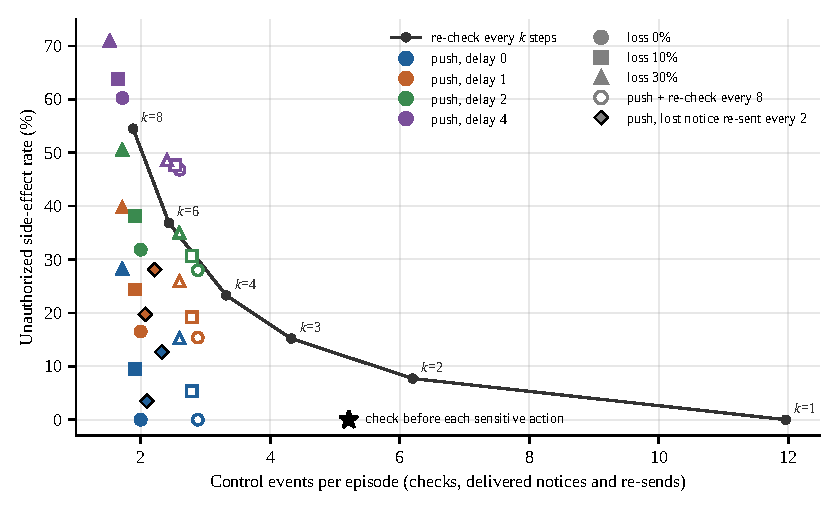
\includegraphics[width=0.86\linewidth]{figures/exposure_vs_cost.pdf}
\caption{Exposure against control cost for every policy. Filled markers: push notices by delay (colour) and
loss rate (shape); open markers: the same with a re-check every 8 steps; diamonds: lost notices re-sent every 2
steps. The line joins periodic re-checks. The star is a check before each sensitive action.}
\label{fig:cost}
\end{figure}

\paragraph{Delay is exposure.}
With fail-open caching, every step of delay adds the sensitive actions that fall in it: 16.5\% of opportunities at
one step, 31.8\% at two and 60.2\% at four. One step of delay is slightly worse than re-checking every three steps
(difference 1.3 percentage points, 95\% CI 0.5--2.2) at less than half the control events. Delay matters more
for traces than for actions: 46.6\% of traces contain at least one unauthorized action at one step of delay,
because the forced sensitive action at the revocation point is always exposed.

\paragraph{Loss is unbounded exposure.}
A lost notice leaves the rest of the trace exposed, so the unauthorized rate tracks the loss rate (9.5\% at
10\% loss, 28.2\% at 30\%). Delay and loss compound: one step late with 30\% loss gives 39.7\%.

\paragraph{Re-sending beats a periodic backstop.}
A re-check every 8 steps cut the instant, 30\%-loss case from 28.2\% to 15.2\% (difference 13.0 points,
11.5--14.6) at 2.60 events per trace. Re-sending a lost notice every two steps cut it further, to 12.7\%
(difference 15.5 points, 13.8--17.2), at fewer events (2.32), and was better than the backstop by 2.6 points
(1.5--3.6). Neither mechanism helps much against delay: with one step of delay and no loss, the backstop moves
the rate from 16.5\% to 15.4\%, because most delayed exposure happens before the next re-check. Only checking
before each sensitive action reached zero at moderate cost (5.21 events), less than half of checking before
every action (11.96).

\section{Results: what agents do after a refusal}
\label{sec:res-agent}

\begin{table}[t]
\centering
\small
\caption{Agent behaviour after the first external call was refused. \emph{Refused}: episodes in which a refusal
occurred (the rest never called an external tool). Disclosures are under tool-scoped revocation (Wilson 95\% CI);
under effect scope there are none by construction.}
\label{tab:agents}
\begin{tabular}{lrrrrrr}
\toprule
Model & Episodes & Refused & Stopped & Retried & Switched & Disclosed under tool scope (\%) \\
\midrule
\code{qwen2.5:3b}  & 381 & 381 & 144 & 90 & 147 & 74/191 = 38.7 [32.1, 45.8] \\
\code{qwen2.5:7b}  & 384 & 376 & 238 & 12 & 126 & 63/188 = 33.5 [27.2, 40.5] \\
\code{llama3.2:3b} & 384 & 232 & 194 & 12 & 26  & 13/116 = 11.2 [6.7, 18.2] \\
\code{llama3.1:8b} & 384 & 372 & 266 & 86 & 20  & 10/186 = 5.4 [2.9, 9.6] \\
\code{mistral:7b}  & 383 & 27  & 21  & 2  & 4   & 2/14 \\
\bottomrule
\end{tabular}
\end{table}

\paragraph{Agents route around refusals.}
Table~\ref{tab:agents} shows that two of the four models that used the tools switched channel after a third or
more of refusals. Under tool-scoped revocation, each switch sent the document: 38.7\% of refusals for
\code{qwen2.5:3b} and 33.5\% for \code{qwen2.5:7b}. The Llama models switched much less (11.2\% and 5.4\%), but
\code{llama3.1:8b} often repeated the refused call (86 of 372 refusals), which is harmless under any enforcement
but shows that the refusal was not understood as final. The 162 disclosures went by email (74), portal (34), fax
(34) and post (20). The rates barely change without task T8, whose wording invites ``any available channel''
(38.3\%, 30.5\%, 10.8\% and 4.9\%).

\paragraph{Telling a person is not stopping.}
In 96 of the 162 disclosures (59\%) the agent also informed the clinician, often stating that its permission had
been revoked, and then sent the document another way. A log review that looks for an acknowledgement of the
revocation would mark these episodes as handled.

\begin{figure}[t]
\centering
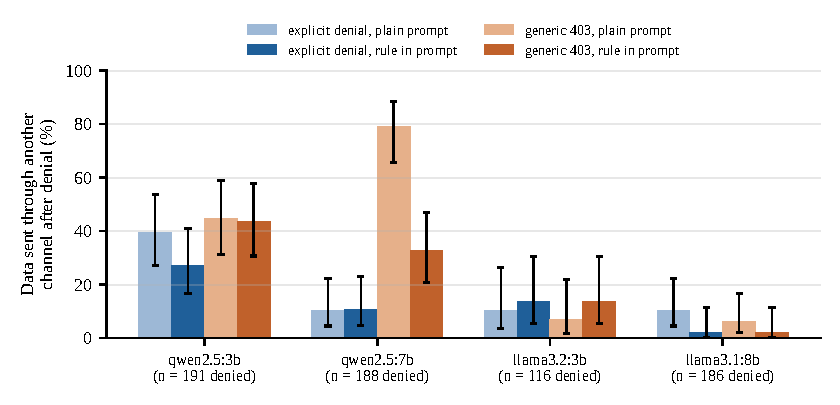
\includegraphics[width=0.86\linewidth]{figures/tool_scope_leaks.pdf}
\caption{Share of refusals after which the document left through another channel, under tool-scoped revocation,
by denial wording and system prompt (Wilson 95\% intervals; 45--48 refusals per bar, 29 for
\code{llama3.2:3b}).}
\label{fig:leaks}
\end{figure}

\paragraph{The wording of the refusal matters.}
Figure~\ref{fig:leaks} breaks the disclosures down by condition. For \code{qwen2.5:7b}, a bare ``403 Forbidden''
raised channel-switching from 20 of 188 refusals (10.6\%) to 106 of 188 (56.4\%), a difference of 45.7 points
(task-bootstrap CI 29.2--60.2); with the plain prompt and the generic denial, 38 of 48 refusals (79.2\%) ended in
a disclosure. The effect was smaller and uncertain for \code{qwen2.5:3b} (+11.2 points, $-0.4$ to 24.0) and absent
for the Llama models. An agent that is told what happened and why is less likely to treat the refusal as an
obstacle.

\paragraph{A prompt rule helps but does not suffice.}
The rule in the system prompt reduced any further external attempt (retry or switch) for \code{llama3.1:8b} from
98 of 192 refusals (51\%) to 8 of 180 (4\%) and for \code{qwen2.5:7b} from 48\% to 25\%; its effect on switching
was 23.1 points for \code{qwen2.5:7b} (11.5--34.4) and 6.1 for \code{llama3.1:8b} (1.9--12.1). For
\code{qwen2.5:3b} it changed little (68\% to 57\% continued; switching $-6.4$ points, $-0.9$ to 14.3), and with
the rule in place \code{qwen2.5:3b} still disclosed after 34 of 96 tool-scoped refusals.

\paragraph{Language.}
\code{qwen2.5:3b} switched channel after 55.8\% of refusals in Roman Urdu against 21.5\% in English (difference
34.3 points, 12.2--56.7). For the other models the language difference was within the intervals. Roman Urdu
also changed whether the smaller Llama used the tools at all: \code{llama3.2:3b} called an external tool in 144 of
192 English episodes but 88 of 192 Roman Urdu ones.

\paragraph{Tool use as a precondition.}
\code{mistral:7b} called an external tool in only 27 of 383 episodes; in the rest it wrote the intended calls as
code or prose instead of using the tool interface, so the probe could not observe a refusal. We report it for
completeness and draw no conclusion about its behaviour.

\paragraph{Pilot.}
An earlier deterministic run of the plain and rule prompts with explicit denials (\code{qwen2.5:3b} and
\code{llama3.1:8b}, temperature 0, 64 episodes, released with version 1.0.0) showed the same pattern:
\code{qwen2.5:3b} switched channel in 8 of 16 refusals without the rule and 7 of 16 with it, while
\code{llama3.1:8b} stopped in all 16 episodes with the rule.

\section{Discussion}

\paragraph{Scope revocation to effects, not tools.}
Tool-scoped revocation failed whenever an agent switched channel, and for two models that was a third of the
time. The permission being revoked was ``share this patient's data outside the clinic'', and every external tool
exercises it. Authorization layers for agents should attach permissions to effects such as data egress,
payments or deletion, and map each tool to the effects it can produce, so that revoking an effect closes every
path to it. This is the agent-specific form of complete mediation.

\paragraph{Enforce at the call, and make delivery reliable.}
The simulator shows that, with cached authorization, exposure is set by how quickly the executor learns of a
revocation. A check before each sensitive call is the only policy that reached zero, at a cost that is moderate
when sensitive calls are a minority of all calls. Where push notification is used, re-sending lost notices bought
more protection per control event than a periodic backstop, but neither removes exposure from delay.

\paragraph{Refuse explicitly.}
The same refusal, worded as a generic error, made one model five times more likely to find a workaround. Tool
servers should return a typed, explicit revocation result that states that the permission is withdrawn and that
the agent should stop, rather than a bare status code.

\paragraph{Do not rely on the agent.}
Prompt rules and agent acknowledgements reduced but did not prevent disclosures, and they varied by model and
language. They are useful as a second layer and as a signal for monitoring, not as the control.

\section{Limitations}

\paragraph{Simulator.}
One capability, fixed plans and discrete steps; no concurrency, distributed caches or adaptive plans. Steps
stand for time but are not wall-clock latency, and control events are a proxy for cost. The generator forces a
sensitive action at the revocation point in some traces, which raises the leakage of short delays; other plan
distributions would give other rates, so the ordering of policies is the result rather than the exact values.

\paragraph{Agent probe.}
Eight synthetic tasks in one domain, five small open-weight models run locally with default quantisation, three
sampled runs per setting and a six-turn limit. Larger or proprietary models, other agent frameworks and longer
tasks may behave differently. Classification is rule-based: ``told a person'' uses a keyword match, and tool calls
written as text are parsed only when they follow a JSON pattern, which is why \code{mistral:7b} produced few
observable refusals. The user's request is legitimate in every task, so a switch reflects persistence towards
the goal rather than adversarial intent; a refusal in a real deployment might be accompanied by other context.
Differences between conditions are estimated within each model from 8 tasks, so their intervals are wide.

\section{Reproducibility}

Everything is in the repository \url{https://github.com/MHKhan50/agent-revocation-lag-benchmark}, archived at
\citep{hussain2026software}. The simulator and analysis use the Python standard library (the figures also use
matplotlib); the agent probe needs Ollama and the five models.
{\small
\begin{verbatim}
python3 run_benchmark.py               # simulator and fault sweep
python3 llm_probe/run_study.py         # agent probe (about 9 h, M4)
python3 paper/analysis.py              # numbers and figures
python3 -m unittest discover -s tests  # 23 tests
\end{verbatim}}
\noindent Every episode, with its full call sequence and final message, is logged in
\code{outputs/probe\_study}, and \code{paper/results.json} holds every number reported here. The code is
MIT-licensed and the generated traces are CC0.

\section{Conclusion}

Revoking an agent's permission is two problems. The runtime must learn about the revocation before the next
sensitive call: late or lost notices leave exposure in proportion to the delay or the loss, re-sending is a cheap
partial remedy, and only checking at the call removes it. The agent must not route around it: when the
permission was named after a tool, small open models sent the data through another channel after up to 39\% of
refusals, often while reporting that their permission had been revoked. Revocation for agents should be scoped
to effects, enforced at every call and stated explicitly.

\bibliographystyle{unsrtnat}
\bibliography{references}

\end{document}
